%----------------------------------------------------------------------------------------
%    PACKAGES AND THEMES
%----------------------------------------------------------------------------------------

\documentclass[aspectratio=169,xcolor=dvipsnames]{beamer}
\usetheme{SimpleDarkBlue}

\usepackage[utf8]{inputenc}
\usepackage{verbatim}
\usepackage{hyperref}
\usepackage{graphicx} % Allows including images
\usepackage{tikz}
\usetikzlibrary{arrows.meta,positioning}
\usepackage{booktabs} % Allows the use of \toprule, \midrule and \bottomrule in tables
\usepackage{lmodern} % Use Latin Modern fonts (provides bold sans-serif)


%----------------------------------------------------------------------------------------
%    TITLE PAGE
%----------------------------------------------------------------------------------------

\title{Physics-informed digital twin for wind turbine main bearing fatigue}

\author{Alexis GONIN \and Tanguy PIERRE}

\institute
{
    UFR Maths, Master CSMI \\
}
\date{May 28, 2025} % Date, can be changed to a custom date

%----------------------------------------------------------------------------------------
%    PRESENTATION SLIDES
%----------------------------------------------------------------------------------------
\begin{document}
% Page de titre personnalisée : titre centré, logo Unistra en bas à droite
\begin{frame}[plain]
    \vfill
    \centering
    % centre verticalement la page de titre
    	\titlepage
    \vfill
    % logo placé en overlay en bas à droite
    \begin{tikzpicture}[remember picture,overlay]
        \node[anchor=south east,xshift=-0.5cm,yshift=0.5cm] at (current page.south east) {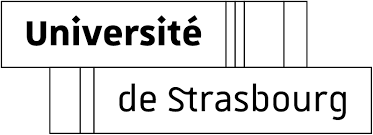
\includegraphics[height=1.8cm]{include/logo-Unistra.jpg}};
    \end{tikzpicture}
\end{frame}

\begin{frame}{Table of Contents}
    % Throughout your presentation, if you choose to use \section{} and \subsection{} commands, these will automatically be printed on this slide as an overview of your presentation
    \tableofcontents
\end{frame}

%------------------------------------------------
\section{Problem and context}
%------------------------------------------------
\begin{frame}{Problem and context}
    \begin{itemize}
        \item Bearing fatigue is a major cause of wind turbine failures, leading to significant downtime and repair costs.
        \item As wind turbines are often located in remote or offshore areas, accessing them for maintenance can be challenging and expensive.
    \end{itemize}
\end{frame}

\section{Objectives of the digital twin}
\begin{frame}{Objectives of the digital twin}
    \begin{itemize}
        \item Predict potential failures in wind turbine main bearings.
        \item Optimize maintenance schedules based on real-time data.
        \item Reduce operational costs through improved efficiency.
    \end{itemize}
\end{frame}


%------------------------------------------------
\section{Pipeline}
%------------------------------------------------
\begin{frame}{Pipeline}
\vfill
\centering
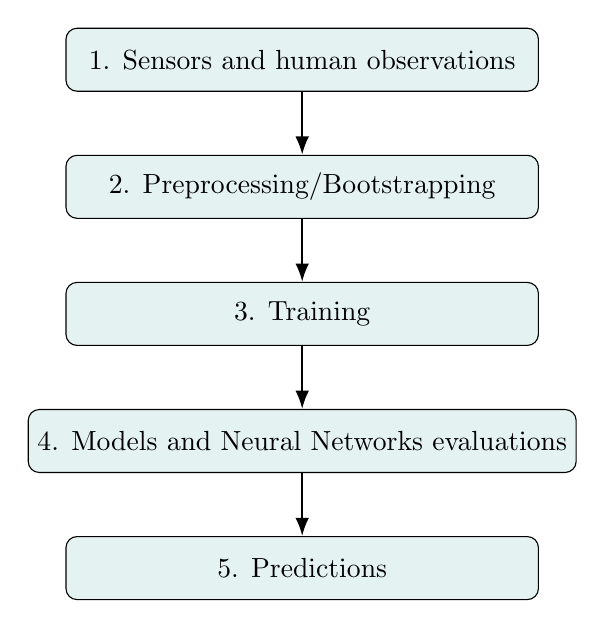
\begin{tikzpicture}[
    stage/.style={rectangle, draw=black, fill=teal!10, rounded corners, minimum width=6cm, minimum height=8mm, align=center},
    arr/.style={-{Latex}, thick},
    node distance=8mm
]
% use relative positioning so the whole diagram can be centered by \centering
\node[stage] (S1) {1. Sensors and human observations};
\node[stage, below=of S1] (S2) {2. Preprocessing/Bootstrapping};
\node[stage, below=of S2] (S3) {3. Training};
\node[stage, below=of S3] (S4) {4. Models and Neural Networks evaluations};
\node[stage, below=of S4] (S5) {5. Predictions};

\draw[arr] (S1.south) -- (S2.north);
\draw[arr] (S2.south) -- (S3.north);
\draw[arr] (S3.south) -- (S4.north);
\draw[arr] (S4.south) -- (S5.north);
\end{tikzpicture}
\vfill
\end{frame}

\section{Methods and models}
\begin{frame}{Methods and models}
    \begin{figure}
        \centering
        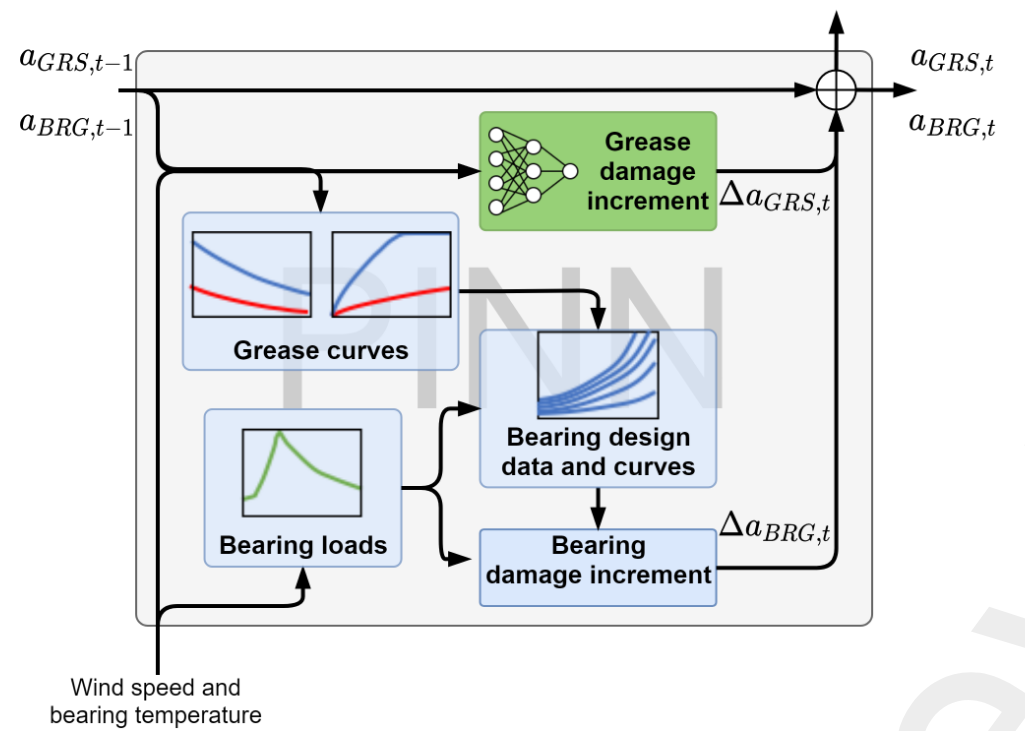
\includegraphics[width=0.6\textwidth]{include/PINN.png}
        \label{fig:pinn}
        \caption{Hybrid physics-informed neural network modeling using recurrent neural networks. Blue boxes represent reduced-order physics-informed kernels and green boxes are data-driven kernels. \cite{YUCESAN2023110921}}
    \end{figure}
\end{frame}

\subsection{Reduced-order physics-informed kernels for bearing fatigue}
\begin{frame}{Reduced-order physics-informed kernels for bearing fatigue}
    \begin{align}
    \Delta a_{\mathrm{BRG}}(t)
    &= \frac{1}{c_1\,c_2(t)}\,P(t)^{C_{1}^{10^3}}, \\[4pt]
    P(t) &= f_1\big(V_W(t)\big), \\[4pt]
    c_2(t) &= f_2\big(P(t),\,\eta_c(t),\,\nu(t)\big), \\[4pt]
    \eta_c(t) &= f_3\big(\nu(t),\,a_{GRS}(t)\big), \\[4pt]
    \nu(t) &= f_4\big(T_{\mathrm{BRG}}(t),\,a_{GRS}(t)\big).
    \end{align}
    with $a_{\mathrm{BRG}}$ the bearing degradation; $a_{\mathrm{GRS}}$ the grease degradation; $c_1$ a factor based on reliability level; $c_2$ an adjustment factor based on lubricant condition (see Fig. 3b); $P$ the dynamic bearing load (see Fig. 3a); $C$ the design load rating; $\eta_c$ the grease contamination factor; $\nu$ the grease viscosity; $V_W$ the wind speed; $T_{\mathrm{BRG}}$ the bearing temperature; $f_1\ldots f_4(\cdot)$ functions defining the models for different components of the bearing damage.
\end{frame}

\subsection{ Physics-informed Neural Network Design for grease Fatigue Estimation}
\begin{frame}{Physics-informed Neural Network Design for grease Fatigue Estimation}
    Grease degradation is evaluated using a neural network.
    \begin{equation}
    \Delta a_{\mathrm{GRS}}(t) \;=\; \mathrm{MLP}\big(V_W(t),\,T_{\mathrm{BRG}}(t),\,a_{\mathrm{GRS}}(t-1);\;\mathbf{w},\,\mathbf{b}\big)
    \end{equation}
\end{frame}

\section{Datas}
\begin{frame}{Datas}
    \begin{itemize}
        \item SCADA (supervisory control and data acquisition); available on board; wind speed and bearing temperature; measured every 10 minutes but no history available. $\rightarrow$ Can be used for  online evaluations.
        \item NREL database: wind speed and ambient temperature every hour for 7 years $\rightarrow$ Can be used for offline Training.
        \item NREL database is used to artificially create SCADA data for 30 simulated years via bootstrapping strategies.
        \item History of grease quality inspection done by humans are available to train the neural network.
    \end{itemize}
\end{frame}

\subsection{Hypothetical data budget table}
\begin{frame}{Data budget table}
Hypothetical example for one wind turbine with 4 thermometers and 1 anemometer. Note that 1 anemometer can be used for several wind turbines in a wind farm.
\vfill 
\centering
\small
\begin{tabular}{l r r r r r l}
\toprule
Sensor & \# & Freq. (m/hour) & Size (B/sample) & bitrate (B/hour) & Volume/day (kB) \\
\midrule
thermometer  & 4  & 6 & 8       & 192  & 4,608  \\
anemometer   & 1  & 6 & 8       & 48   & 1,152  \\
\bottomrule
\end{tabular}
\end{frame}

\section{Verification and validation}
\begin{frame}{Verification and validation}

\end{frame}

\section{Transferability and deployment}
\begin{frame}{Transferability and deployment}

\end{frame}

\section{Perspectives and limitations}
\begin{frame}{Perspectives and limitations}

\end{frame}

\section{References}
\begin{frame}{References}
\bibliographystyle{plain}
    \bibliography{biblio}
    \cite{YUCESAN2023110921}
\end{frame}


\end{document}